\documentclass[conference, 10pt]{IEEEtran}
%\IEEEoverridecommandlockouts
% The preceding line is only needed to identify funding in the first footnote. If that is unneeded, please comment it out.
\usepackage{cite}
\usepackage{amsmath,amssymb,amsfonts}
\usepackage{algorithmic}
\usepackage{graphicx}
\usepackage{textcomp}
\usepackage{xcolor}
\usepackage[colorlinks = true,
            linkcolor = blue,
            urlcolor  = blue,
            citecolor = blue,
            anchorcolor = blue]{hyperref}
\usepackage[spanish,activeacute]{babel}

\def\BibTeX{{\rm B\kern-.05em{\sc i\kern-.025em b}\kern-.08em
    T\kern-.1667em\lower.7ex\hbox{E}\kern-.125emX}}
\begin{document}

\title{Problem Set 3: Ganancias con Machine Learning\\}

\author{\IEEEauthorblockN{Andrea Margarita Beleño}
\IEEEauthorblockA{200620739\\
E-mail:a.beleno@uniandes.edu.co}
\and
\IEEEauthorblockN{María Valeria Gaona}
\IEEEauthorblockA{202214418\\
E-mail:mv.gaona@uniandes.edu.co}
}

\maketitle

\begin{abstract}
El precio de las viviendas cuenta con diferentes factores que se tienen en consideración para establecer un valor. Por lo tanto, contar con un modelo en el que se identifiquen dichas características principales es fundamental para poder generar una predicción lo más óptima posible. Por lo tanto, en el siguiente documento se realizará el modelo de predicción para los precios de las viviendas por medio de Random Forest. El link al Github del presente taller, se encuentra en el siguiente enlace:\url{https://github.com/mvgaona/Problem-Set-3}\\

\end{abstract}


\section{Introducción}
El precio de una vivienda está dado por diferentes factores como el área total, el número de baños, número de habitaciones, la distancia a puntos importantes de la ciudad, entre otros elementos que explican dicho valor. Además, cada ciudad cuenta con diferentes características que aportan a que los vendedores decidan establecer un precio. Sin embargo, se puede generar un modelo en donde se pueda observar el efecto de cada una de esas características esenciales que da el valor de un inmueble y así, tanto el vendedor como el comprador conoce cada uno de estos impactos para realizar futuras compras y/o ventas de inmuebles. \
Por otra parte, generar una predicción de estos valores es una herramienta óptima para conocer el comportamiento económico de una sociedad y además, cada individuo puede obtener información valiosa para la toma de decisiones a mediano o largo plazo. De acuerdo con lo anterior, en el presente documento se presenta el proceso de la limpieza de datos pertinente para continuar con la caracterización de las variables fundamentales y así, realizar el modelo de predicción de los precios de las viviendas en la localidad de Chapinero en la ciudad de Bogotá y en el área del poblado en Medellín, ambas ciudades Colombianas.


\section{Datos} \label{AA}

El precio de una vivienda puede estar dados por diferentes factores, tanto económicos como sociales. En el caso Colombiano, estos precios pueden estar influenciados por elementos propios de la vivienda y a su vez, por elementos geoespaciales, como la distancia a diversos lugares públicos (Bares, transporte público, etc). Para realizar un modelo de predicción de precios de la vivienda, es necesario contar con las variables determinantes y relevantes del precio, para que este modelo sea robusto, pero no se incurran en gastos que entorpezcan la investigación. En el presente modelo de predicción se tomó en cuenta solo los datos de  las viviendas ubicadas en las localidades objetivo (Chapinero y Poblado) y el total de datos (Base de entrenamiento y base de testeo) es de 24.843 viviendas. \
Dentro del proceso de recolección de datos puede ocurrir que no se encuentren toda la información necesaria, ya sea porque la base de datos no provee dicha información o, por el contrario, no se pudo recolectar toda la información de cada vivienda. Es por eso que es necesario realizar un proceso de limpieza y recuperación de datos. Se realizaron diversos procesos para poder contar con toda la información:
\begin{enumerate}
	\item Se cuenta con variables las cuales ya tienen la información completa, por lo tanto no es necesario realizar ningún tratamiento:\\
\textit{-Ubicación}: La ubicación del inmueble en el modelo será esencial para el análisis ya que se analizarán dos localidades de dos ciudades diferentes y los precios de las ciudades si bien están dados por características similares, el costo de vida por ciudad también influye en el valor de la vivienda. Esta variable es categórica, la cual presenta la proporción de cada ciudad dentro de la base de datos, presentada en el Cuadro ~\ref{tab_1}.\\
\textit{-	Tipo de propiedad}: Si la propiedad es un apartamento o si es una casa influye sustancialmente en el precio, ya que el área de una casa suele ser más grande, cuenta con más oportunidad de reformas y espacios más amplios de esparcimiento. Esta variable categórica cuenta con la proporción  presentada en el Cuadro ~\ref{tab_2}.\\
 \item	De acuerdo con los valores proporcionados de cada variable, se generó la comparación entre dicha información y los valores hallados por medio de la inspección de la descripción de cada inmueble, generando las siguientes variables sin información faltante:\\
\textit{- Habitaciones}: El número de habitaciones de la vivienda es determinante en el precio de la misma, ya que se puede contar con un aproximado del espacio y de cuántos individuos puedes vivir con la mayor calidad de vida posible, es decir, entre más habitaciones, el precio del inmueble tiende a incrementarse. Por lo tanto, dentro del análisis descriptivo de este predictor se encuentra que es  una variable numérica, la cual presenta los valores respecto al número de habitaciones consignados en el Cuadro ~\ref{tab_3}.\\
\textit{-	Cantidad de baños}: Este es otro factor de decisión importante en el precio del inmueble, ya que sin baños, los individuos no pueden satisfacer las necesidades básicas de aseo. Por lo tanto es necesario contar con al menos un baño y con ello, se puede identificar que a medida que aumentan la cantidad de baños, el precio de igual manera se verá afectado e incrementará. De acuerdo con lo anterior, se observa que en la variable numérica se evidencian los valores respecto a el análisis de todos los inmuebles consignados en el Cuadro ~\ref{tab_4}. \
 \item De acuerdo con la información proporcionada por la descripción de cada inmueble, se generaron las siguientes variables:\\
\textit{-	Ascensor}: Si el inmueble cuenta con ascensor o no es determinante en el caso de los apartamentos de pisos altos, es por eso que se considera un predictor importante del modelo, ya que quienes viven en pisos más altos, buscan apartamentos donde tenga ascensor y a su vez, el precio aumenta si el inmueble cuenta con esta herramienta de desplazamiento dentro del edificio. Dentro del análisis descriptivo de la variable, es posible identificar que es una variable categórica de 2 niveles: 1 y 0, donde 1 corresponde a si el inmueble cuenta con ascensor y 0 si no. Esta variable cuenta con la proporción presentada en el Cuadro Cuadro ~\ref{tab_5}. Los inmuebles que no cuentan con ascensor también contar con apartamentos que no cuentan con uno y casas que no necesitan, las cuales no lo necesitan.\\
\textit{-	Parqueadero}: En la actualidad, gran parte de los individuos cuentan con uno o más carros, por lo tanto, es necesario que el inmueble cuente con al menos un parqueadero para que el individuo no incurra en gastos adicionales en encontrar un lugar seguro para su(s) carro(s), por lo tanto, si el inmueble incluye al menos un garaje, el precio de la vivienda tenderá a aumentar su valor. Por otra parte, de acuerdo con el análisis descriptivo, se identifica que esta es una variable categórica de dos niveles, en donde 1 hace referencia a que la casa o el apartamento cuenta con al menos un parqueadero y 0 que no lo hace. La proporción de inmuebles que cuentan con al menos un parqueadero se presenta en el Cuadro ~\ref{tab_6}. La proporción puede estar dada debido a que algunos vendedores no ofrecieron dicha información, por ejemplo.
\item De acuerdo con la ubicación geoespacial, se pueden recuperar datos por medio el hallazgo de características similares de otras viviendas y dicho promedio, adjuntarlo al inmueble que no cuenta con información. Ya que, al estar en un perímetro cercano, los inmuebles suelen presentar características similares.\\
-\textit{	Área}: El área de un inmueble es fundamental para conocer el precio del mismo, ya que a medida que el área aumente, este también aumenta. Esto se da debido a que un espacio amplio permite contar con un mayor número de habitaciones, baños, una cocina más amplia y demás espacios de esparcimiento. Además, permite más posibilidades de remodelación y de inversión. Por lo tanto, ante la variable numérica presentada, en el Cuadro ~\ref{tab_7}  se encuentran los valores respecto al análisis de las viviendas.

\item	Por medio de la ubicación geoespacial se pueden hallar diferentes variables que pueden predecir los precios de las viviendas, ya que existen puntos importantes de las ciudades, las cuales entre menos distancia exista entre el inmueble y el punto, el valor del inmueble aumenta\\
-\textit{	Transporte público}: Contar con al menos un transporte público cerca de la vivienda es fundamental para poder analizar la facilidad vial y que tan alejado puede estar del resto de la ciudad. Por lo tanto, esta variable presenta la distancia mínima que tiene el inmueble con al menos un medio de transporte público, ya que a medida que esta distancia sea más corta, el precio puede incrementarse. De acuerdo al análisis, se evidencian las distancias mínimas presentadas en el Cuadro ~\ref{tab_8}.\\
\textit{-Bares}: La distancia mínima a bares es otro factor a tener en cuenta, ya que, en general, este tipo de establecimiento hace que pueda generar incomodidad a los habitantes en las horas de la noche. Por lo tanto, al estar cada vez más alejados de un bar, el comprador puede estar más interesado en el inmueble. De acuerdo con la variable numérica, se presentan las distancias mínimas en el Cuadro ~\ref{tab_9}.\\
\textit{-	Parques}: La distancia mínima a por lo menos un parque es otro predictor relevante dentro del modelo, ya que, en general, los individuos buscan tener un espacio verde y de recreación cerca, ya sea porque dentro del hogar tienen niños los cuales puedan entretenerse, mascotas que necesiten espacio libre para derrochar su energía o cumplir sus necesidades fisiológicas o porque los compradores también desean un espacio al aire libre para su propio entrenamiento. Por lo tanto, a medida que esta distancia va disminuyendo, el precio del inmueble tiende a incrementar. La variable numérica presenta la descripción estadística en el Cuadro ~\ref{tab_10}.
\end{enumerate}

\section{Mapas}
Los  mapas de la localidad de Chapinero en Bogotá y El Poblado en Medellín, presentados en las Figuras ~\ref{fig_1} y ~\ref{fig_2}, evidencian la distribución de bares, estaciones de buses, y parques que se encuentran en cada uno de los sectores, junto con las viviendas que se encuentran en las localidades anteriormente mencionadas. Esto permite contar con un análisis gráfico de cada vivienda y así, un comprador, por ejemplo, puede contar con información gráfica que le permite tomar decisiones de manera informada.
\begin{figure}[htbp]
\centerline{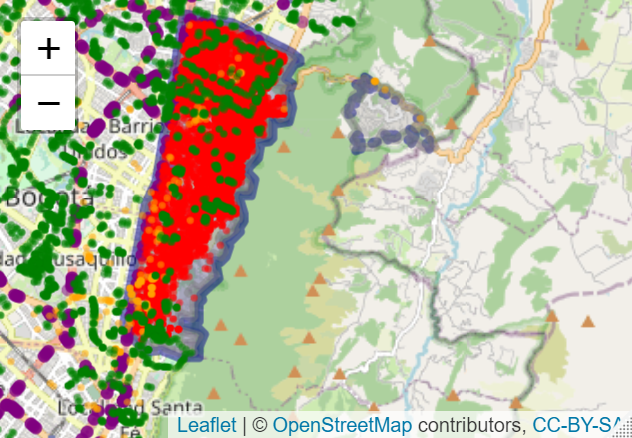
\includegraphics[width=0.4\textwidth]{../Vistas/Mapa_Chapinero_2.2.png}}
\caption{Mapa Chapinero, Bogotá- \textit{Polígono color azul, apartamentos en rojo, transp. público en morado, parques en verde y naranja para bares}}
\label{fig_1}
\end{figure}

\begin{figure}[htbp]
\centerline{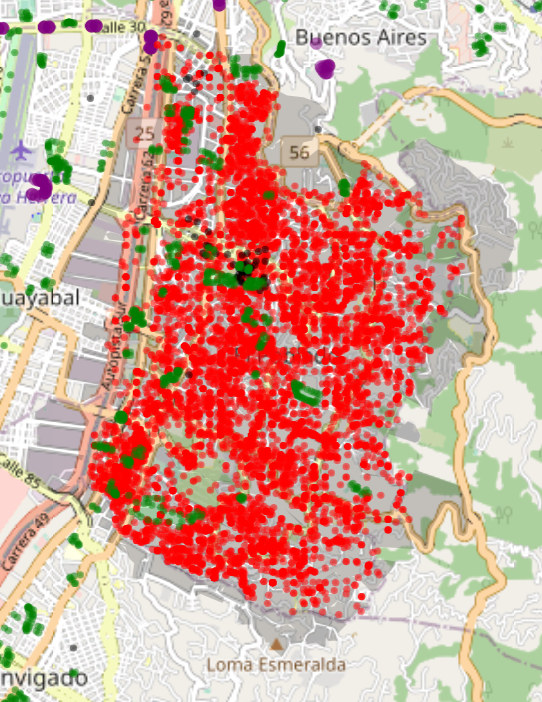
\includegraphics[width=0.4\textwidth]{../Vistas/MapaPoblado1.png}}
\caption{Mapa El Poblado, Medellín- \textit{Polígono color azul, apartamentos en rojo, transp. público en morado, parques en verde y negro para bares}}
\label{fig_2}
\end{figure}

\section{Modelo y Resultados}
Con base en las variables presentadas en la sección \ref{AA}, se procedió a realizar varios modelos para determinar cuál era el más apropiado para realizar la predicción de precio de viviendas. Se analizó la posibilidad de partir la base \textit{train} en un \textit{subtrain} y \textit{subtest}, sin embargo, teniendo en cuenta que la base de \textit{test} original cuenta con 11.150 observaciones, realizar la subdivisión de \textit{train} en un menor número de muestras, podría ir en perjuicio de la predicción, al utilizar incluso menos datos que la base \textit{test} principal, por lo cual, se decidió realizar implementar los modelos sobre la base \textit{train} reducida. En primera instancia, se realizó un modelo de regresión con \textit{OLS} (modelo 1), tomando las 10 variables presentadas anteriormente, luego, se realizó la regularización de Lasso para la regresión OLS U (modelo 2). Adicionalmente, se realizaron los modelos \textit{Random Forest} (modelo 3) y \textit{XGBoost} (modelo 4), teniendo en cuenta las variables mencionadas anteriormente. A manera ilustrativa, se presentará el modelo OLS utilizado contemplando las 10 variables.
\begin{multline*}
Price= \beta_{0}+\beta_{1}Ubicacion+\beta_{2}Tipo-vivienda+\beta_{3}Habitac.+\\
\beta_{4}Banios+\beta_{5}Ascensor+\beta_{6}Parqueadero+\beta_{7}Area+\\
\beta_{8}Dist.Transp.Pub.+\beta_{9}Dist.bares+\beta_{10}Dist.parques+u \\
\end{multline*}
Luego de correr los modelos, la significancia de las variables variaba de un modelo a otro, por ejemplo, para \textit{OLS} existían 5 variables más significativas para el modelo vs las que se obtuvieron en \textit{Random Forest} que fueron 6 con mayor peso para el modelo. A continuación se presentarán las variables relevantes obtenidas en \textit{OLS}:
\begin{itemize}
\item \textit{Habitación}, \textit{Baños}, \textit{Área}, \textit{Área}, \textit{Distancia a bares}, \textit{Distancia a transporte público} 
\end{itemize}
A continuación se presentarán las variables relevantes obtenidas en \textit{Random Forest}:
\begin{itemize}
\item \textit{Habitación}, \textit{Baños}, \textit{Área}, \textit{Área}, \textit{Distancia a bares}, \textit{Distancia a transporte público},  \textit{Distancia a parques}
\end{itemize}
Utilizando las variables presentadas anteriormente, se corrieron los modelos mencionados incialmente (\textit{OLS}, \textit{Lasso}, \textit{Random Forest}, \textit{XGBoost}, es decir, se contó con 16 modelos. Al hacer la comparación de la raíz cuadrada del MSE, se obtuvo que para los modelos incluyendo las 10 variables se presentó el menor MSE. El modelo de \textit{Random Forest} fue entrenado variando el número de árboles, para el cual se obtuvo un valor de $n.trees=1000$.\\
En la Figura ~\ref{fig_3} , se presenta la comparación de los primeros 4 modelos con las 10 variables en términos de la raíz del MSE para tener una primera aproximación de cuál modelo escoger. Ahora bien, existen otros temas relevantes a tener en cuenta para decidir cuál modelo se debe escoger para realizar la predicción, como lo es la relación de dinero para compra vs. la cantidad de viviendas compradas, que se escoge el de menor ratio, porque para esos casos se compran más viviendas a un costo menor. Se realizó la comparación de cada set de modelos, con las 10, 5 y 6 variables, de lo cual se obtuvo la información presentada en el Cuadro ~\ref{tab_11}. Lo anterior, para concluir que el mejor modelo para realizar la predicción fue el de \textit{Random Forest} con 10 variables. Finalmente, la predicción obtenida se guardó en el archivo .csv solicitado.
\\

\begin{figure}[htbp]
\centerline{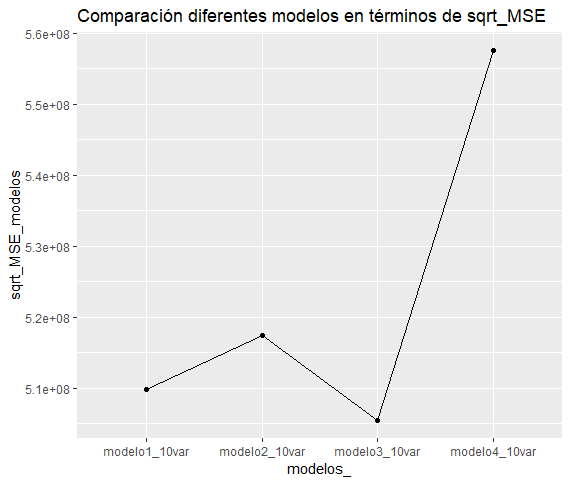
\includegraphics[width=0.4\textwidth]{../Vistas/Comp_MSE_modelos_var_10.png}}
\caption{Comparación MSE modelos para obtener \textit{price}}
\label{fig_3}
\end{figure}

\section{Conclusiones y recomendaciones}
\begin{itemize}
\item Fue un reto bastante interesante obtener los datos geográficos para utilizarlos como predictores, teniendo en cuenta 
\item Se encontraron diferencias significativas en cuanto a la predicción por clasificación y por regresión a través del ingreso. Los parámetros utilizados para realizar la clasificación de Pobre o No Pobre, puede incidir.
\item La regresión del Ingreso presentó un MSE alto para todos los modelos, motivo por el cual, se puede estar dando este resultado en donde hay pobres clasificados como no pobres.
\item Los resultados más aceptables para el ejercicio fueron los que tuvieron en cuenta mayor cantidad de variables para obtener la predicción (variable dependiente).
\end{itemize}




\appendix[Cuadros de Variables descriptivas]
\begin{table}[htbp]
\caption{Cuadro descriptivo \textit{Ubicación}}
\begin{center}
\begin{tabular}{|c|c|}
\hline
\multicolumn{2}{|c|}{\textbf{Ubicación}} \\
\cline{1-2} 
\hline
 Bogotá D.C.&Medellín\\
 14.244&10.599\\
 (57,34\%)&(42,7\%)\\
 
	\hline
\end{tabular}
\label{tab_1}
\end{center}
\end{table}

\begin{table}[htbp]
\caption{Cuadro descriptivo \textit{Tipo de vivienda}}
\begin{center}
\begin{tabular}{|c|c|}
\hline
\multicolumn{2}{|c|}{\textbf{Tipo de Vivienda}} \\
\cline{1-2} 
\hline
 Casa&Apartamento\\
 2.038&22.805\\
 (8,2\%)&(91,8\%)\\
 
	\hline
\end{tabular}
\label{tab_2}
\end{center}
\end{table}

\begin{table}[htbp]
\caption{Cuadro descriptivo \textit{Habitaciones}}
\begin{center}
\begin{tabular}{|c|c|c|c|}
\hline
\multicolumn{4}{|c|}{\textbf{Habitaciones}} \\
\cline{1-4} 
\hline
 Mín&Media&Máx.&Moda\\
\hline
 1&3&11&3\\
 	\hline
\end{tabular}
\label{tab_3}
\end{center}
\end{table}

\begin{table}[htbp]
\caption{Cuadro descriptivo \textit{Número de baños}}
\begin{center}
\begin{tabular}{|c|c|c|c|}
\hline
\multicolumn{4}{|c|}{\textbf{Número de baños}} \\
\cline{1-4} 
\hline
 Mín&Media&Máx.&Moda\\
\hline
 1&3&13&2\\
 	\hline
\end{tabular}
\label{tab_4}
\end{center}
\end{table}

\begin{table}[htbp]
\caption{Cuadro descriptivo \textit{Ascensor}}
\begin{center}
\begin{tabular}{|c|c|}
\hline
\multicolumn{2}{|c|}{\textbf{Ascensor}} \\
\cline{1-2} 
\hline
 Tiene ascensor&No tiene ascensor\\
 19.388 (78,04\%)&5.455(21,96\%)\\
  
	\hline
\end{tabular}
\label{tab_5}
\end{center}
\end{table}

\begin{table}[htbp]
\caption{Cuadro descriptivo \textit{Parqueadero}}
\begin{center}
\begin{tabular}{|c|c|}
\hline
\multicolumn{2}{|c|}{\textbf{Parqueadero}} \\
\cline{1-2} 
\hline
 Tiene parqueadero&No tiene parqueadero\\
 7.885(31,74\%)&16.958(68,26\%)\\
  
	\hline
\end{tabular}
\label{tab_6}
\end{center}
\end{table}

\begin{table}[htbp]
\caption{Cuadro descriptivo \textit{Área}}
\begin{center}
\begin{tabular}{|c|c|c|c|}
\hline
\multicolumn{4}{|c|}{\textbf{Área (m\^{2})}} \\
\cline{1-4} 
\hline
 Mín&Media&Máx.&Moda\\
\hline
 74,06&286,75&3.940,14&193,7414\\
 	\hline
\end{tabular}
\label{tab_7}
\end{center}
\end{table}


\begin{table}[htbp]
\caption{Cuadro descriptivo \textit{Transporte Público-TP}}
\begin{center}
\begin{tabular}{|c|c|c|c|}
\hline
\multicolumn{4}{|c|}{\textbf{Distancia TP (m)}} \\
\cline{1-4} 
\hline
 Mín&Media&Máx.&Moda\\
\hline
 4,397&1.519,834&4.472,144&2.168,091\\
 	\hline
\end{tabular}
\label{tab_8}
\end{center}
\end{table}

\begin{table}[htbp]
\caption{Cuadro descriptivo \textit{Distancia bares}}
\begin{center}
\begin{tabular}{|c|c|c|c|}
\hline
\multicolumn{4}{|c|}{\textbf{Distancia bares (m)}} \\
\cline{1-4} 
\hline
 Mín&Media&Máx.&Moda\\
\hline
 2,101&1.694,033&3.062,209&487,8808\\
 	\hline
\end{tabular}
\label{tab_9}
\end{center}
\end{table}

\begin{table}[htbp]
\caption{Cuadro descriptivo \textit{Distancia parques}}
\begin{center}
\begin{tabular}{|c|c|c|c|}
\hline
\multicolumn{4}{|c|}{\textbf{Distancia parques (m)}} \\
\cline{1-4} 
\hline
 Mín&Media&Máx.&Moda\\
\hline
 0,4975&230,5497&1.567,7500&478,1448\\
 	\hline
\end{tabular}
\label{tab_10}
\end{center}
\end{table}

\begin{table}[htbp]
\caption{Evaluación Modelos Variables 10}
\begin{center}
\begin{tabular}{|c|c|c|c|c|c|}
\hline
\multicolumn{4}{|c|}{\textbf{Distancia parques (m)}} \\
\cline{1-4} 
\hline
\textbf{OLS}&\textbf{Lasso}&\textbf{RF, n=5}&\textbf{RF, n=1000}\\
\hline
 0,4975&230,5497&1.567,7500&478,1448\\
 	\hline
\end{tabular}
\label{tab_10}
\end{center}
\end{table}


% Table created by stargazer v.5.2.3 by Marek Hlavac, Social Policy Institute. E-mail: marek.hlavac at gmail.com
% Date and time: lun., jul. 25, 2022 - 10:28:47 p. m.
\begin{table}[!htbp] \centering 
  \caption{} 
  \label{} 
\begin{tabular}{@{\extracolsep{5pt}}lc} 
\\[-1.8ex]\hline 
\hline \\[-1.8ex] 
 & \multicolumn{1}{c}{\textit{Dependent variable:}} \\ 
\cline{2-2} 
\\[-1.8ex] & price \\ 
\hline \\[-1.8ex] 
 factor(Medellin)1 & $-$787,636,375.000$^{***}$ \\ 
  & (61,083,213.000) \\ 
  & \\ 
 factor(Apto)1 & 207,203,199.000$^{***}$ \\ 
  & (34,086,495.000) \\ 
  & \\ 
 factor(parqueaderoT)1 & $-$63,801,814.000$^{***}$ \\ 
  & (13,453,959.000) \\ 
  & \\ 
 factor(ascensorT)1 & 124,196,586.000$^{***}$ \\ 
  & (14,752,857.000) \\ 
  & \\ 
 bathrooms & 153,238,037.000$^{***}$ \\ 
  & (5,325,096.000) \\ 
  & \\ 
 habitaciones & 317,659,483.000$^{***}$ \\ 
  & (7,138,710.000) \\ 
  & \\ 
 min\_dist\_bar\_ & $-$13,904.660 \\ 
  & (25,102.360) \\ 
  & \\ 
 min\_dist\_transp\_ & 526,386.800$^{***}$ \\ 
  & (16,935.530) \\ 
  & \\ 
 min\_dist\_park & $-$720,497.400$^{***}$ \\ 
  & (62,258.320) \\ 
  & \\ 
 surface\_new\_3 & 123,250.800$^{***}$ \\ 
  & (36,015.530) \\ 
  & \\ 
 Constant & $-$463,068,798.000$^{***}$ \\ 
  & (44,297,272.000) \\ 
  & \\ 
\hline \\[-1.8ex] 
Observations & 13,693 \\ 
R$^{2}$ & 0.370 \\ 
Adjusted R$^{2}$ & 0.369 \\ 
Residual Std. Error & 720,926,630.000 (df = 13682) \\ 
F Statistic & 802.327$^{***}$ (df = 10; 13682) \\ 
\hline 
\hline \\[-1.8ex] 
\textit{Note:}  & \multicolumn{1}{r}{$^{*}$p$<$0.1; $^{**}$p$<$0.05; $^{***}$p$<$0.01} \\ 
\end{tabular} 
\end{table} 


\end{document}
